\documentclass{standalone}
\usepackage{pgfplots}
\usepackage{xcolor}
\pgfplotsset{compat=1.17}

% Auburn colors
\definecolor{auburnorange}{RGB}{232, 119, 34}
\definecolor{auburnblue}{RGB}{12, 35, 64}

\begin{document}
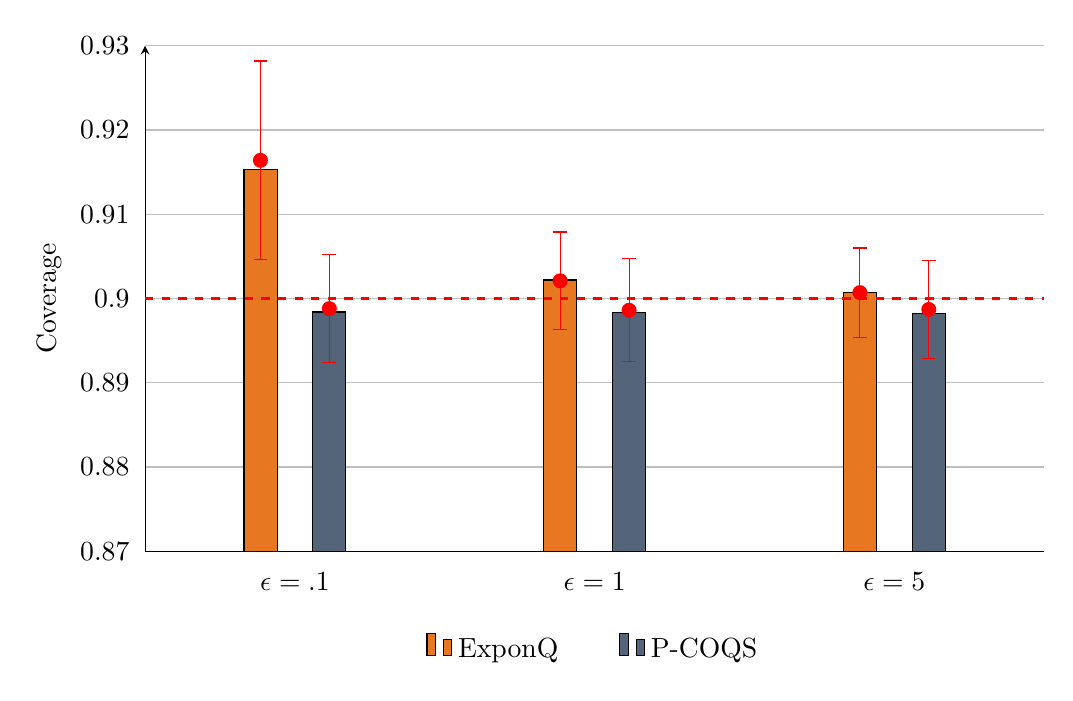
\begin{tikzpicture}
\begin{axis}[
    ybar,
    bar width=12pt,
    enlargelimits=0,
    ymin=0.87, ymax=0.93,
    ylabel={Coverage},
    xtick={1,2,3},
    xticklabels={$\epsilon=.1$, $\epsilon = 1$, $\epsilon=5$},
    legend style={at={(0.5,-0.15)}, anchor=north, legend columns=2, /tikz/every even column/.append style={column sep=2em}, draw=none },
    ymajorgrids=true,
    axis x line*=bottom,
    axis y line=left,
    tick style={draw=none},
    width=13cm,
    height=8cm,
]

% --- ExponQ bars at positions 0.85, 1.85, 2.85 ---
\addplot+[
    draw=black,
    fill=auburnorange,
%    error bars/.cd,
%        y dir=both, y explicit,
]
coordinates {
    (0.95, 0.9153) 
    (1.95, 0.9022)
    (2.95, 0.9007)
};

% --- P-COQS bars at positions 1.15, 2.15, 3.15 ---
\addplot+[
    draw=black,
    fill=auburnblue!70,
%    error bars/.cd,
%        y dir=both, y explicit,
]
coordinates {
    (1.05, 0.8984)
    (2.05, 0.8983)
    (3.05, 0.8982)
};

% --- Mean red points ---
\addplot+[
	color = red,
    only marks,
    mark=*,
    mark color = red,
    mark size=2.5pt,
    error bars/.cd,
    		y dir=both, y explicit,
] coordinates {
    (0.885, 0.9164) +- (0, 0.0118) 
    (1.115, 0.8988)  +- (0, 0.0064) 
    (1.885, 0.9021) +- (0, 0.0058)
    (2.115, 0.8986) +- (0, 0.0061)
    (2.885, 0.9007) +- (0, 0.0053)
    (3.115, 0.8987) +- (0, 0.0058)
};

% Horizontal dashed target line at 0.9
\addplot[
    red,
    dashed,
    thick,
    sharp plot
] coordinates {
    (0.5, 0.9)
    (3.5, 0.9)
};

\legend{ExponQ\hspace{5em}, P-COQS}
\end{axis}
\end{tikzpicture}
\end{document}
